\chapter{Lec 15 - 2-Approximation Algorithm for Metric TSP}

\section{Metric TSP: A 2-Approximation Algorithm}
For the Vertex Cover problem we used the concept of maximal matching to find a 2-approximation algorithm, for Metric TSP we'll use \textbf{Minimum Spanning Tree}. The total MST weight gives a lower bound on the length of an optimal traveling-salesman tour. We shall then use the minimum spanning tree to create a tour whose cost is no more than twice of the minimum spanning tree’s weight, as long as the cost function satisfies the triangle inequality.\newline\newline
\textbf{Intuition:}
First of all, we need to transform the tree in a cycle. In order to do this, we can use the \textbf{Preorder} visit of the MST.
\begin{algorithm}
\caption{PREORDER}\label{PREORDER}
    \begin{algorithmic}[1]
    \Procedure{PREORDER($T, v$)}{}
        \State visit($v$)
        \If{$v$ is internal}
            \For{\textbf{each} $u \in \text{children($v$)}$}
                \State PREORDER($T, u$)
            \EndFor
        \EndIf
        \Return
    \EndProcedure   
    \end{algorithmic}
\end{algorithm}\newline\newline
\textbf{Example:}\newline\newline
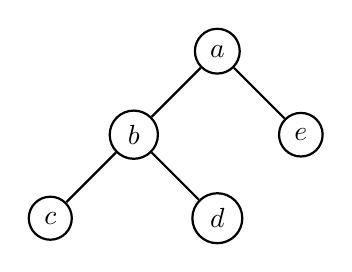
\begin{tikzpicture}[node distance={15mm}, thick, main/.style = {draw, circle}] 
            \node[main] (a) {$a$}; 
            \node[main] (b) [below left of=a] {$b$}; 
            \node[main] (e) [below right of=a] {$e$}; 
            \node[main] (c) [below left of=b] {$c$}; 
            \node[main] (d) [below right of=b] {$d$};

            \draw (a) -- (b); 
            \draw (a) -- (e); 
            \draw (b) -- (c);
            \draw (b) -- (d);
\end{tikzpicture}\newline\newline
\textbf{Preorder} list: $a, b, c, d, e$.\newline\newline
Note that the result is \textbf{not} a cycle since $e$ and $a$ are not connected. We can simply solve this problem by adding the edge $(e, a)$ to the Preorder list and make it a Hamiltonian circuit. We are free to add every edge we want because the graph is complete by definition.\newline\newline
The resulting cycle of the MST above is the following:\newline\newline
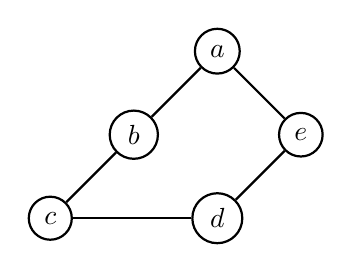
\begin{tikzpicture}[node distance={15mm}, thick, main/.style = {draw, circle}] 
            \node[main] (a) {$a$}; 
            \node[main] (b) [below left of=a] {$b$}; 
            \node[main] (e) [below right of=a] {$e$}; 
            \node[main] (c) [below left of=b] {$c$}; 
            \node[main] (d) [below right of=b] {$d$};

            \draw (a) -- (b); 
            \draw (b) -- (c);
            \draw (c) -- (d);
            \draw (d) -- (e);
            \draw (e) -- (a);
\end{tikzpicture}\newline\newline
Now we can define an algorithm that exploits this idea:
\begin{algorithm}
\caption{Approx\_Metric\_TSP}\label{ApproxMetricTSP}
    \begin{algorithmic}[1]
    \Procedure{Approx\_Metric\_TSP($G$)}{}
        \State $V = \{v_1, v_2, ..., v_n\}$
        \State $r = v_1 \quad \text{// root from which Prim is run}$
        \State $T^* = Prim(G, r)$
        \State $<v_{i_1}, v_{i_2}, ..., v_{i_n}> = H' = PREORDER(T^*, r)$
        \State \textbf{return} $<H', v_{i_1}>\, = H \quad \text{// close the cycle}$
    \EndProcedure   
    \end{algorithmic}
\end{algorithm}\newline\newline
This algorithm uses Prim as a subroutine to compute the MST.
\begin{center}
    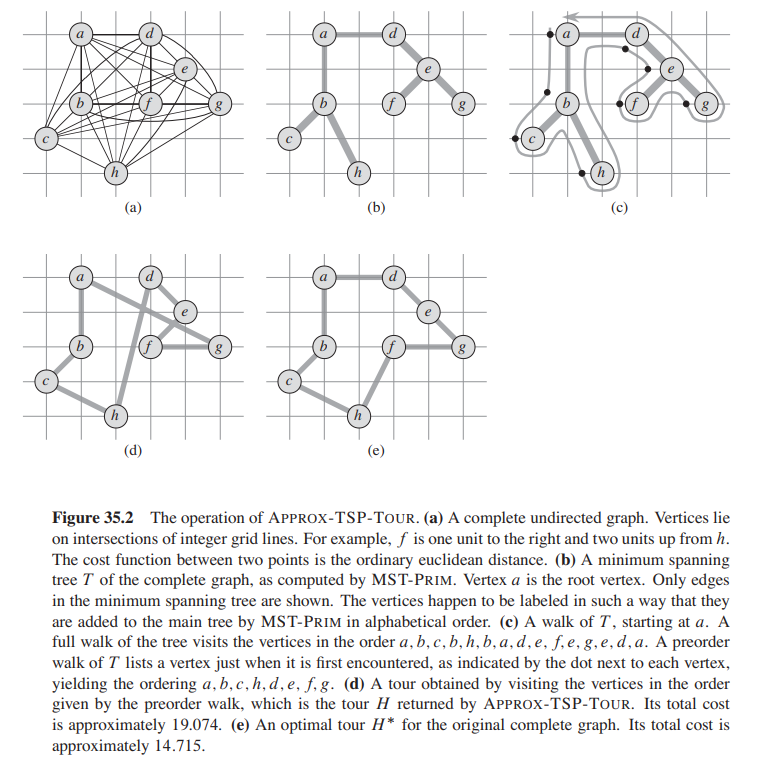
\includegraphics[scale=0.7]{images/Approx-metric-tsp.png}
\end{center}

\subsection{Analysis of the cost of $H$}
Let $H^*$ denote an optimal tour for the given set of vertices.
\begin{enumerate}
    \item The cost of $T^*$ is a lower bound to the cost of $H^*$.
    \[w(H^*) \geq w(T^*)\]
    This is because we obtain a spanning tree by deleting any edge from a tour, and each edge cost is non-negative. Therefore, the weight of the minimum spanning tree $T^*$ provides a lower bound to the cost of an optimal tour.

    \item  Then we have to find an upper bound to the cost of $H$ (the returned solution). We want to prove that:
    \[w(H) \leq 2w(T^*) \leq 2w(H^*)\]
    \textbf{Definition:} given a tree, a \textbf{full preorder chain} is a list with repetitions of the vertices of the tree which identifies the vertices reached from the recursive calls of $PREORDER(T, u)$.\newline\newline
    \textbf{Example}:\newline\newline
    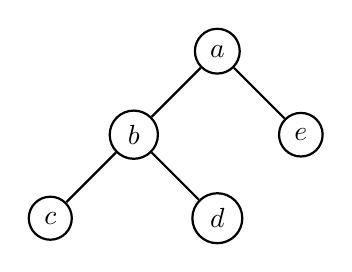
\begin{tikzpicture}[node distance={15mm}, thick, main/.style = {draw, circle}] 
            \node[main] (a) {$a$}; 
            \node[main] (b) [below left of=a] {$b$}; 
            \node[main] (e) [below right of=a] {$e$}; 
            \node[main] (c) [below left of=b] {$c$}; 
            \node[main] (d) [below right of=b] {$d$};

            \draw (a) -- (b); 
            \draw (a) -- (e); 
            \draw (b) -- (c);
            \draw (b) -- (d);
    \end{tikzpicture}\newline\newline
    \textbf{full preorder chain:} $a, b, c, b, d, b, a, e, a$\newline\newline
    Since the full preorder chain traverses every edge of $T^*$ exactly twice, we have:
    \[w(f.p.c) = 2w(T^*) \leq 2w(H^*)\]
    Unfortunately, the f.p.c is generally not a tour, since it visits some vertices more than once. By \textbf{the triangle inequality}, however, we can delete a visit to any vertex from f.p.c and the cost does not increase. By repeatedly applying this operation, we can remove from f.p.c. all but the first visit to each vertex (except for the last occurrence of the root). This is like adding a \textit{shortcut} between vertices that does not increase the cost. In our example:
    \[2w(T^*) = w(<a, b, c, b, d, b, a, e, a>)\]
    \[\geq w(<a, b, c, d, b, a, e, a>)\]
    \[ ... \]
    \[\geq w(<a, b, c, d ,e, a>)\]
    Then, we have that:
    \[2w(T^*) \geq w(H)\]
\end{enumerate}
\textbf{Putting all together:}
\begin{enumerate}
    \item $w(H^*) \geq w(T^*)$
    \item $2w(T^*) \geq w(H)$
\end{enumerate}
This implies that:
\[2w(H^*) \geq 2w(T^*) \geq w(H)\]
\[\frac{w(H)}{w(H^*)} \leq 2\]

